\section{Первая программа}
\subsection{Базовый вариант}
\begin{code}
	\captionof{listing}{Первая программа, базовый вариант}
	\inputminted
	[
	frame=single,
	framerule=0.5pt,
	framesep=10pt,
	fontsize=\small,
	tabsize=4,
	linenos,
	numbersep=5pt,
	xleftmargin=10pt,
	]
	{c}
	{code/1_1.c}
\end{code}

\begin{figure}[!hbpt]
	\centering
	
\includegraphics[width=\textwidth]{image/1-1}
	\caption{Вывод программы}
\end{figure}
\newpage
С помощью системного вызова open() создается дескриптор открытого файла (только для чтения). Системный вызов open() возвращает индекс в массиве fd структуры files\_struct.  Библиотечная функция fdopen() возвращает указатели на struct FILE (fs1 и fs2), которые ссылаются на дескриптор, созданный системным вызовом open(). Далее создаются буферы buff1 и buff2 размером 20 байт. Для дескрипторов fs1 и fs2 функцией setvbuf() задаются соответствующие буферы и тип буферизации \_IOFBF.

Далее fscanf() выполняется в цикле поочерёдно для fs1 и fs2. 
При первом вызове fscanf() для fs1 в буфер buff1 считаются первые 20 символов. Значение f\_pos в структуре struct\_file открытого увеличится на 20. В переменную c записывается символ ’a’ и выводится с помощью fprintf(). При первом вызове fscanf() для fs2 в буфер buff2 считываются оставшиеся в файле символы (в переменную с записывается символ ’u’).

В цикле символы из buff1 и buff2 будут поочередно выводиться до тех пор, пока символы в одном из буферов не закончатся. Тогда на экран будут последовательно выведены оставшиеся символы из другого буфера. 

\newpage
\subsection{Связи структур}
\begin{figure}[!h!]
	\centering
	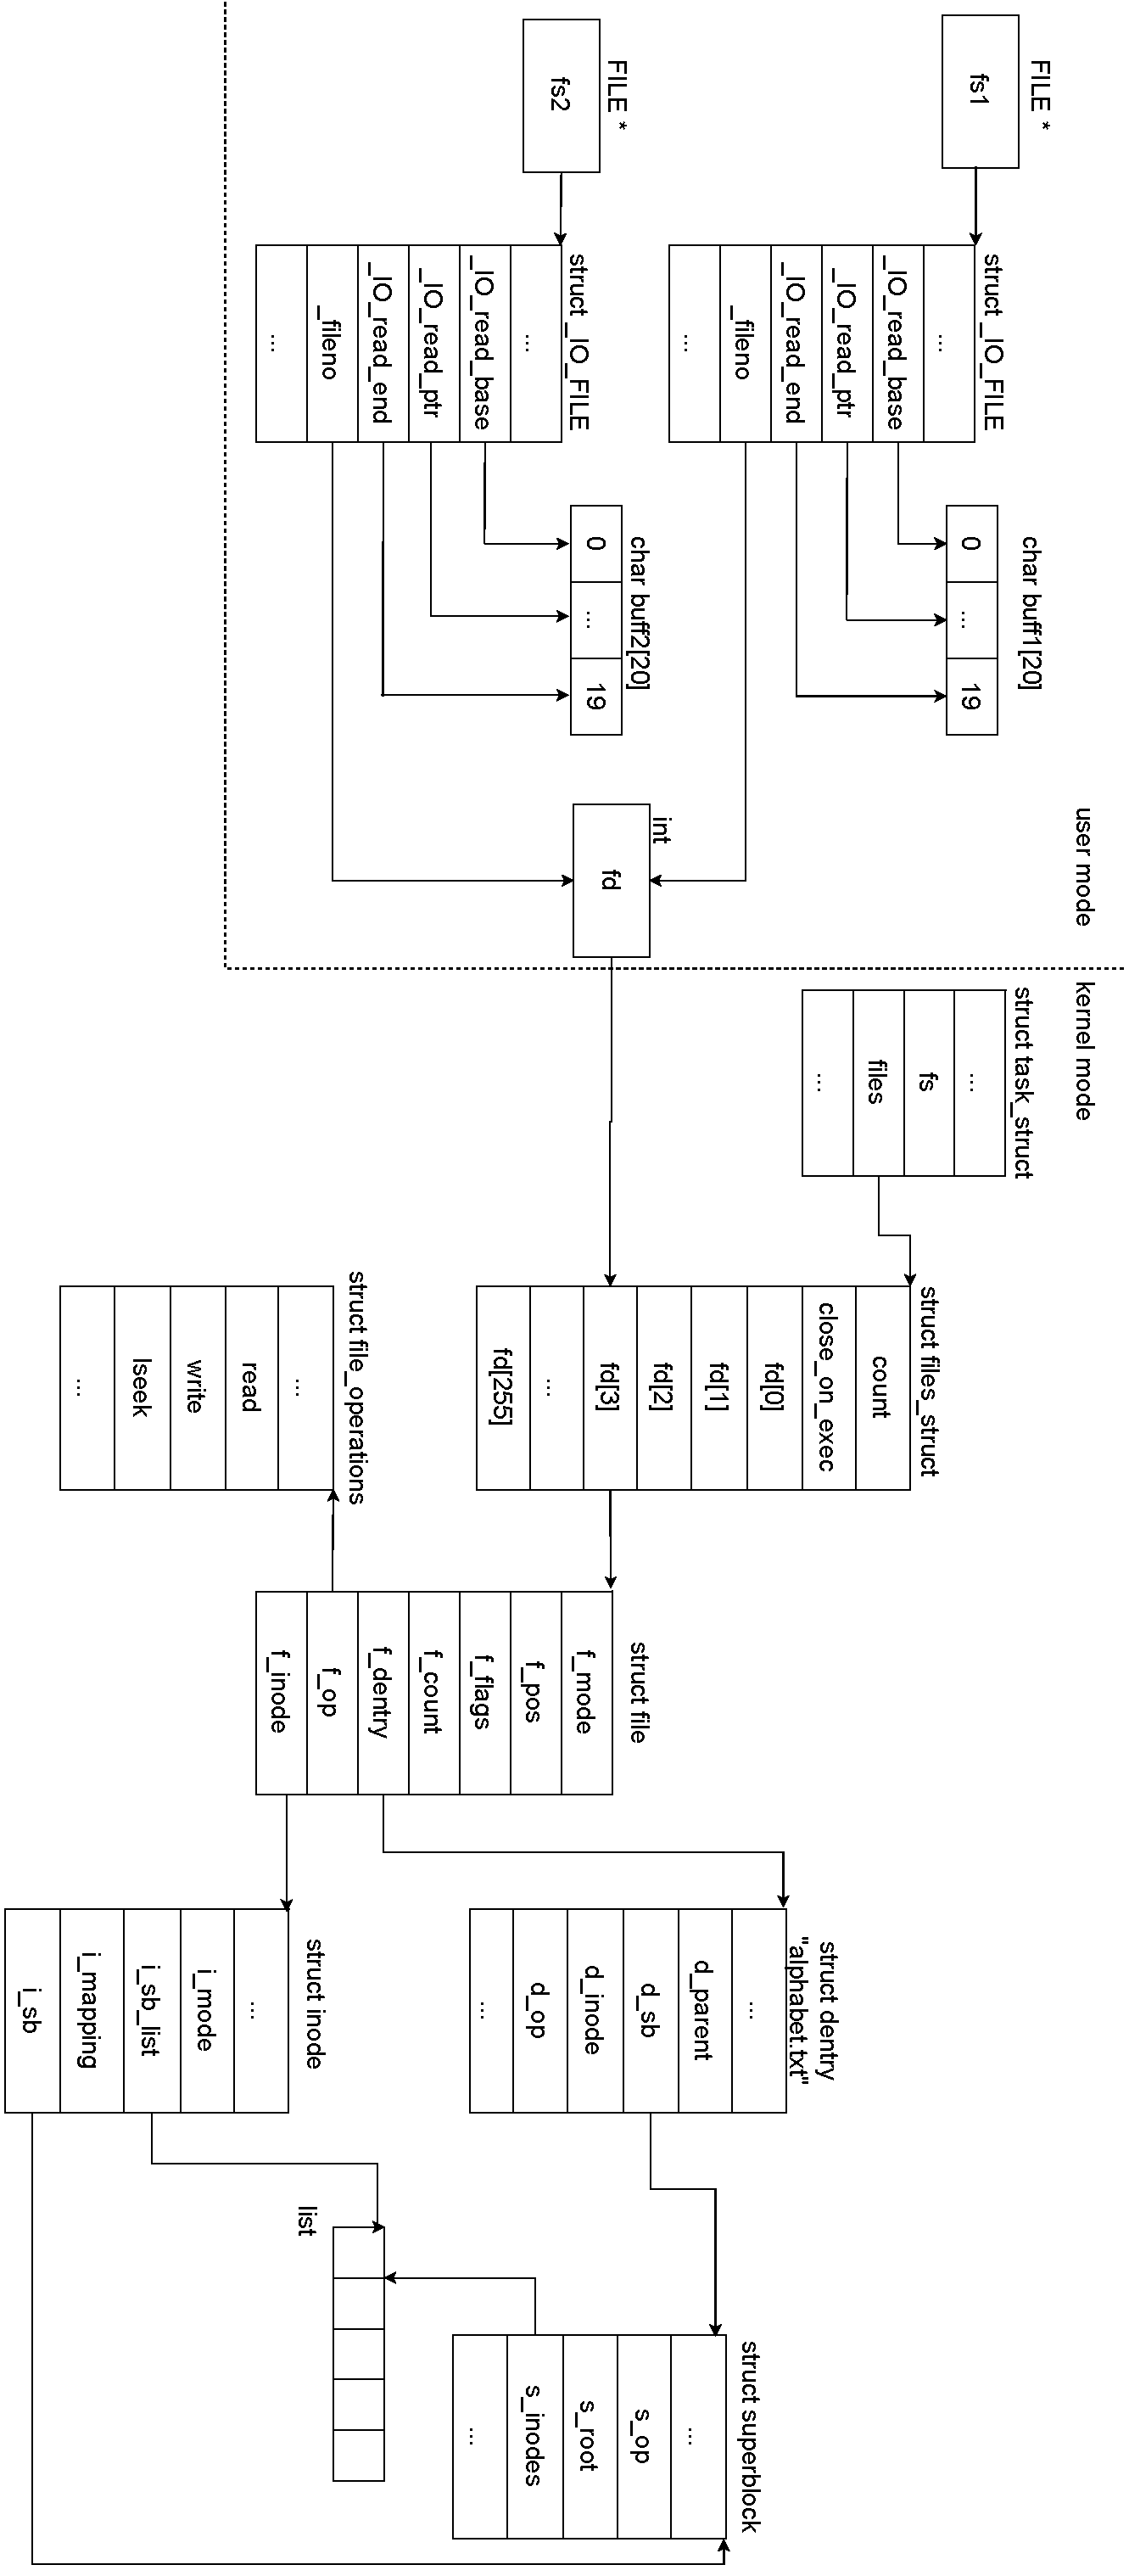
\includegraphics[width=100mm]{image/d1}
	\caption{Связи структур в первой программе}
\end{figure}
\clearpage

\subsection{Многопоточный вариант}
\begin{code}
	\captionof{listing}{Первая программа с созданием двух дополнительных потоков}
	\inputminted
	[
	frame=single,
	framerule=0.5pt,
	framesep=10pt,
	fontsize=\small,
	tabsize=4,
	linenos,
	numbersep=5pt,
	xleftmargin=10pt,
	]
	{c}
	{code/1_2.c}
\end{code}

\begin{figure}[!h]
	\centering
	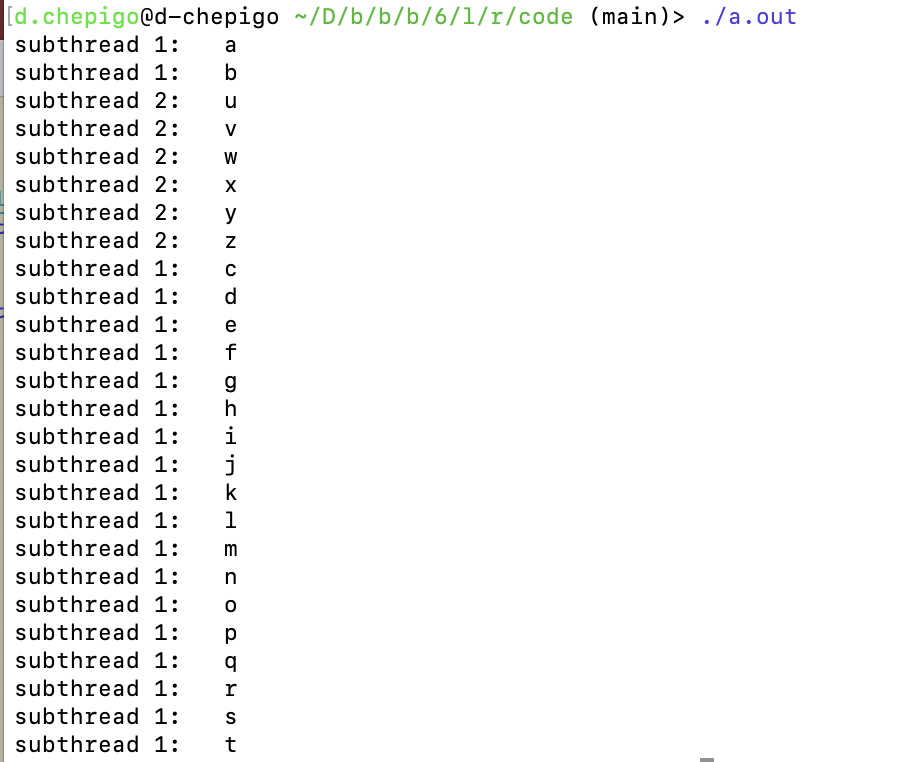
\includegraphics[width=\textwidth]{image/1-2}
	\caption{Вывод программы}
\end{figure}
\newpage

В однопоточной программе в цикле поочередно выводятся символы из buff1 и buff2, в то время как в многопоточной программе главный поток на- чинает вывод раньше, так как для дополнительного потока сначала затрачи- вается время на его создание, и только потом начинается вывод.
При создании дополнительных потоков связи структур не изменяются, так как ресурсами (в том числе и открытыми файлами) владеет процесс.


